\documentclass[12pt]{report}
\usepackage[utf8]{inputenc}
\usepackage[T1]{fontenc}
\usepackage[french]{babel}
\usepackage{graphicx}
\graphicspath{{./}{images/}{public/images/}{../public/images/}}
\makeatletter
\def\input@path{{./}{images/}{public/images/}{../public/images/}}
\makeatother
\usepackage{xcolor}
\usepackage{tikz}
\usepackage{geometry}
\usepackage{anyfontsize}
\usepackage{setspace}
\usepackage{lmodern}
\usepackage{microtype} 
\usepackage{shadowtext}
\usepackage{background}
\usepackage{float}
\usepackage[outline]{contour}
\usepackage{multirow}
\usepackage{array}
\usepackage{booktabs} 
\usepackage{caption}
\usepackage{parskip}

\DeclareCaptionFont{ninept}{\fontsize{9}{11}\selectfont}
\DeclareCaptionLabelSeparator{frenchcolon}{~: }
\captionsetup[figure]{
  font=ninept,
  labelfont=it,
  textfont=it,
  labelsep=frenchcolon
}
\DeclareCaptionLabelSeparator{endash}{\space\textendash\space}
\captionsetup[table]{
  font=ninept,
  labelfont=it,
  textfont=it,
  name=Table,
  labelsep=endash
}
\usepackage{hyperref}
\usepackage{wrapfig}
\usepackage{enumitem}
\usepackage{amsmath}
\usepackage{amssymb}
\usepackage{titlesec}

% Define a minimal neutral palette (grayscale)
\definecolor{primary}{RGB}{34,34,34}
\definecolor{secondary}{RGB}{102,102,102}
\definecolor{accent}{RGB}{140,140,140}
\definecolor{darkgray}{RGB}{66, 66, 66}
\definecolor{mediumgray}{RGB}{117, 117, 117}
\definecolor{lightgray}{RGB}{245, 245, 245}
\definecolor{bordercolor}{RGB}{100, 100, 100}

\renewcommand{\familydefault}{\rmdefault}
\setstretch{1.2}

\pagecolor{white}
\color{black}

% Page configuration — marges réduites, pas de top excessif
\geometry{
  a4paper,
  left=2cm,
  right=2cm,
  top=2cm,
  bottom=2cm,
  includeheadfoot
}

% Réduire l'espace en haut des chapitres
\titlespacing*{\chapter}{0pt}{-5pt}{20pt}

% Forcer une marge supérieure plus petite pour les pages de chapitre (report)
\makeatletter
\def\@makechapterhead#1{%
  \vspace*{-25\p@}   % or -30\p@, -1cm, etc.
  {\parindent \z@ \raggedright \normalfont
    \ifnum \c@secnumdepth >\m@ne
      \huge\bfseries \@chapapp\space \thechapter
      \par\nobreak
      \vskip 20\p@
    \fi
    \interlinepenalty\@M
    \Huge \bfseries #1\par\nobreak
    \vskip 30\p@
  }}

\def\@makeschapterhead#1{%
  \vspace*{-25\p@}   % or -30\p@, -1cm, etc.
  {\parindent \z@ \raggedright
    \normalfont
    \interlinepenalty\@M
    \Huge \bfseries #1\par\nobreak
    \vskip 30\p@
  }}
\makeatother

\backgroundsetup{
  scale=1,
  angle=0,
  opacity=0.05,
}

% Logos inline sans légende (petits, sans numérotation figure)
\newcommand{\inlinetech}[3]{%
  \begin{minipage}[t]{0.18\textwidth}
    \centering
    \IfFileExists{images/#1}{\includegraphics[width=1.8cm,height=1.8cm,keepaspectratio]{images/#1}}{%
      \IfFileExists{#1}{\includegraphics[width=1.8cm,height=1.8cm,keepaspectratio]{#1}}{\fbox{\rule{0pt}{1.8cm}\rule{1.8cm}{0pt}}}%
    }%
  \end{minipage}\hfill
  \begin{minipage}[t]{0.78\textwidth}
    \textbf{#2}~--- #3
  \end{minipage}\par\medskip
}

% Safe include pour captures d'écran — inclut depuis le dossier images/ si présent
\newcommand{\safeinclude}[2]{%
  \IfFileExists{images/#1}{\includegraphics[width=#2]{images/#1}}{}%
}

\begin{document}

% ============================================================
%  PAGE DE GARDE
% ============================================================
\begin{titlepage}
  \centering 

  \IfFileExists{fste.png}{
\includegraphics[width=0.3\textwidth]{fste.png}}{\fbox{\rule{0pt}{2cm}\rule{0.28\textwidth}{0pt}}}\hspace{1.4cm}
  \IfFileExists{company.png}{\includegraphics[width=0.22\textwidth]{company.png}}{\fbox{\rule{0pt}{2cm}\rule{0.2\textwidth}{0pt}}}\hspace{1cm}
  \IfFileExists{logo.png}{\includegraphics[width=0.31\textwidth]{logo.png}}{\fbox{\rule{0pt}{2cm}\rule{0pt}{2cm}\rule{0.24\textwidth}{0pt}}}

  \vspace{0.6cm}
  {\fontsize{12}{14}\selectfont\textbf{Faculté des Sciences et Techniques d'Errachidia}\par}

  \vspace{2cm}
  {\fontsize{14}{16}\selectfont\textbf{Rapport de projet de fin d'année :}\par}
  \vspace{0.5cm}
  {\fontsize{15}{17}\selectfont\textbf{Cycle d'Ingénieur : Ingénierie Logicielle et Intelligence Artificielle}\par}
  \vspace{1.5cm}
  {\fontsize{16}{18}\selectfont\textbf{Intitulé :}\par}
  \vspace{0.5cm}

  \fboxrule=1.5pt
  \fboxsep=12pt
  {\fbox{\parbox{0.85\textwidth}{\centering
    \vspace{10pt}
    {\fontsize{14}{20}\selectfont\bfseries CONCEPTION ET RÉALISATION DE CINEPASS\par}
    \vspace{5pt}
    {\fontsize{11}{13}\selectfont Plateforme de réservation de billets et gestion de salles de cinéma\par}
    \vspace{10pt}
  }}}

  \vfill


  \noindent
  {\fontsize{12}{14}\selectfont
  \renewcommand{\arraystretch}{0.9}
  \begin{tabular*}{\textwidth}{@{}p{0.66\textwidth}@{\extracolsep{\fill}}>{\raggedleft\arraybackslash}p{0.32\textwidth}@{}}
    $\diamond$ \textbf{Pr Mohammed BOUTALLINE} (FST Errachidia) & \textbf{Encadrant académique} \\
      \vspace{0.01cm}
     $\diamond$ \textbf{Equipe CinePass} &       \vspace{0.01cm}
   \textbf{Maître de stage / Référent projet} \\
    \vspace{0.5cm}
    \textbf{    Réalisé par :}  \textbf{       Yassine EL AOUNI} \\
  \end{tabular*}
  }

  \vspace{2cm}
  {\fontsize{11}{12}\selectfont\textbf{PÉRIODE DU STAGE : 1 JUILLET AU 1 OCTOBRE 2025}\par}
  \vspace{0.5cm}
  {\fontsize{12}{14}\selectfont\textbf{Année universitaire : 2024/2025}\par}
  \vspace{0.5cm}
\end{titlepage}

% ============================================================
\chapter*{Remerciements}
\addcontentsline{toc}{chapter}{Remerciements}

Je tiens à exprimer ma profonde gratitude à mes professeurs, qui m'ont transmis des connaissances précieuses, m'ont guidé tout au long de cette année universitaire et ont contribué de manière déterminante à ma formation.

Je remercie tout particulièrement Pr. Aziz BAATAOUI, mon encadrant académique à la Faculté des Sciences et Techniques d'Errachidia, pour son suivi pédagogique, ses conseils avisés et sa contribution à l'orientation de ce projet.

J'adresse également mes sincères remerciements à l'ensemble des enseignants de la Faculté des Sciences et Techniques d'Errachidia pour leur accompagnement, leur disponibilité et la qualité de leur encadrement.

Je tiens à remercier chaleureusement l'équipe CinePass pour leur accueil et leur suivi technique tout au long de ce projet.

Pour finir, une pensée toute particulière pour ma famille et mes amis, qui m'ont soutenu et encouragé tout au long de cette période. Leur présence a été un moteur essentiel pour mener à bien ce travail.

% ============================================================
\chapter*{Résumé}
\addcontentsline{toc}{chapter}{Résumé}

Ce document présente le travail réalisé dans le cadre de mon Projet de Fin d'Année (PFA) de première année du cycle d'ingénieur en Génie Logiciel et Intelligence Artificielle. Le projet \textbf{CinePass} a consisté en la conception et le développement d'une plateforme complète de billetterie et de gestion de salles de cinéma, permettant la réservation de sièges, la consultation d'horaires et le paiement en ligne.

Sur le plan technique, j'ai développé une interface utilisateur moderne avec React et Vite, en m'appuyant sur une architecture backend en TypeScript (NestJS). L'architecture repose sur une séparation claire des responsabilités, avec des modules dédiés à la gestion des films, des séances, des réservations et des paiements.

Les fonctionnalités implémentées couvrent la recherche et la consultation des films et séances, la sélection interactive des sièges avec validation des disponibilités en temps réel, la gestion des comptes utilisateurs et l'intégration d'un système de paiement. Le document détaille les choix techniques, les défis rencontrés et les solutions apportées, ainsi que les pistes d'amélioration pour l'évolution future de la plateforme.

% ============================================================
\chapter*{Abstract}
\addcontentsline{toc}{chapter}{Abstract}

This document presents the work carried out for my First-Year Engineering Project (PFA) in Software Engineering and Artificial Intelligence. The CinePass project involved the design and development of a complete ticketing and cinema management web platform.

From a technical perspective, I developed a web interface using React and Vite, building upon a NestJS backend. The architecture uses a clear separation of concerns with dedicated modules for films, sessions, reservations and payments.

Implemented features include seat selection with availability checks, user account management and integrated payment flows. This report details the technical choices, encountered challenges and implemented solutions, and proposes improvements for future iterations.

\setcounter{secnumdepth}{3} 

\tableofcontents
\listoffigures
\listoftables

% Liste des abréviations
\chapter*{Liste des abréviations}
\addcontentsline{toc}{chapter}{Liste des abréviations}
\begin{table}[H]
  \centering
  \begin{tabular}{|p{4cm}|p{9cm}|}
    \hline
    \textbf{Abréviation} & \textbf{Signification} \\
    \hline
    API & Application Programming Interface (interface de programmation) \\
    \hline
    SPA & Single Page Application (application monopage) \\
    \hline
    PFA & Projet de Fin d'Année \\
    \hline
    JWT & JSON Web Token (jeton d'authentification) \\
    \hline
    RGPD & Règlement Général sur la Protection des Données \\
    \hline
    UX & Expérience utilisateur (User Experience) \\
    \hline
    UI & Interface utilisateur (User Interface) \\
    \hline
    REST & Representational State Transfer (architecture d'API) \\
    \hline
    WCAG & Directives pour l'accessibilité des contenus web \\
    \hline
  \end{tabular}
  \caption{Principales abréviations utilisées dans ce rapport}
  \label{tab:abreviations}
\end{table}

% ============================================================
%  INTRODUCTION GÉNÉRALE (non numérotée, pas un chapitre)
% ============================================================
\chapter*{Introduction générale}
\addcontentsline{toc}{chapter}{Introduction générale}

Le secteur de la billetterie et de la gestion des salles de cinéma demande des solutions fiables pour gérer les réservations, les ventes et l'expérience spectateur. Le projet \textbf{CinePass} vise à fournir une plateforme centralisée permettant aux utilisateurs de consulter les films, réserver des sièges, et payer en ligne, tout en offrant aux exploitants des outils de gestion des séances et des statistiques d'occupation.

Sur le plan technique, le projet s'appuie sur des choix modernes : une application web monopage (SPA) développée avec React et assemblée avec Vite, un backend en TypeScript et NestJS exposant une API REST, et des principes d'architecture modulaire côté frontend. L'effort a porté sur l'intégration fonctionnelle, la gestion fiable des états (états de réservation en temps réel) et la fiabilité des paiements.

Le développement s'est déroulé selon une approche incrémentale privilégiant l'ajout progressif de fonctionnalités visibles. Ce rapport est structuré en trois chapitres : le premier présente le projet CinePass ; le deuxième couvre l'analyse des besoins et la conception du système ; le troisième expose les choix techniques retenus et les réalisations concrètes obtenues.

% ============================================================
\chapter{Présentation du projet CinePass}

Ce chapitre présente le contexte du projet CinePass, ses objectifs et l'organisation générale des composants logiciels.

\section{Vision globale}

CinePass est une plateforme de billetterie et de gestion de salles de cinéma destinée à simplifier l'achat de billets pour les spectateurs et la gestion des séances pour les exploitants. Elle regroupe la consultation des films, la sélection des séances, la réservation de sièges en temps réel et la gestion des transactions.

Le projet comprend plusieurs volets : une interface d'administration pour gérer les films et les séances, une application web destinée aux utilisateurs finaux, et une application mobile (React Native) pour la consultation et l'achat depuis smartphone.

\section{Objectifs de la plateforme}

Les objectifs principaux sont les suivants : centraliser la vente de billets, offrir une interface de sélection de sièges intuitive, garantir la fiabilité des réservations concurrentes, intégrer des passerelles de paiement sécurisées et fournir des outils d'analyse pour le suivi d'affluence et des ventes.

\section{Périmètre de mon intervention}

Mon intervention s'est concentrée sur le développement du site web utilisateur et sur l'intégration avec l'API backend. Les responsabilités comprenaient l'interface de réservation, la sélection visuelle des sièges, la gestion des sessions utilisateur, et l'intégration du paiement et du suivi des commandes.

\section{Contexte technique du projet}

La stack technique comprend :
\begin{itemize}
  \item \textbf{Frontend :} React 18 + Vite, TypeScript, Tailwind CSS pour le design et une librairie de gestion d'état (Redux Toolkit ou Zustand) selon le module.
  \item \textbf{Backend :} NestJS (TypeScript) exposant des endpoints REST pour la gestion des films, séances, réservations et paiements.
  \item \textbf{Base de données :} MySQL/Postgres selon les besoins de production.
  \item \textbf{Mobile :} Application React Native pour consultation et achat mobile.
\end{itemize}

\begin{figure}[H]
\centering
\IfFileExists{architecture-overview.png}{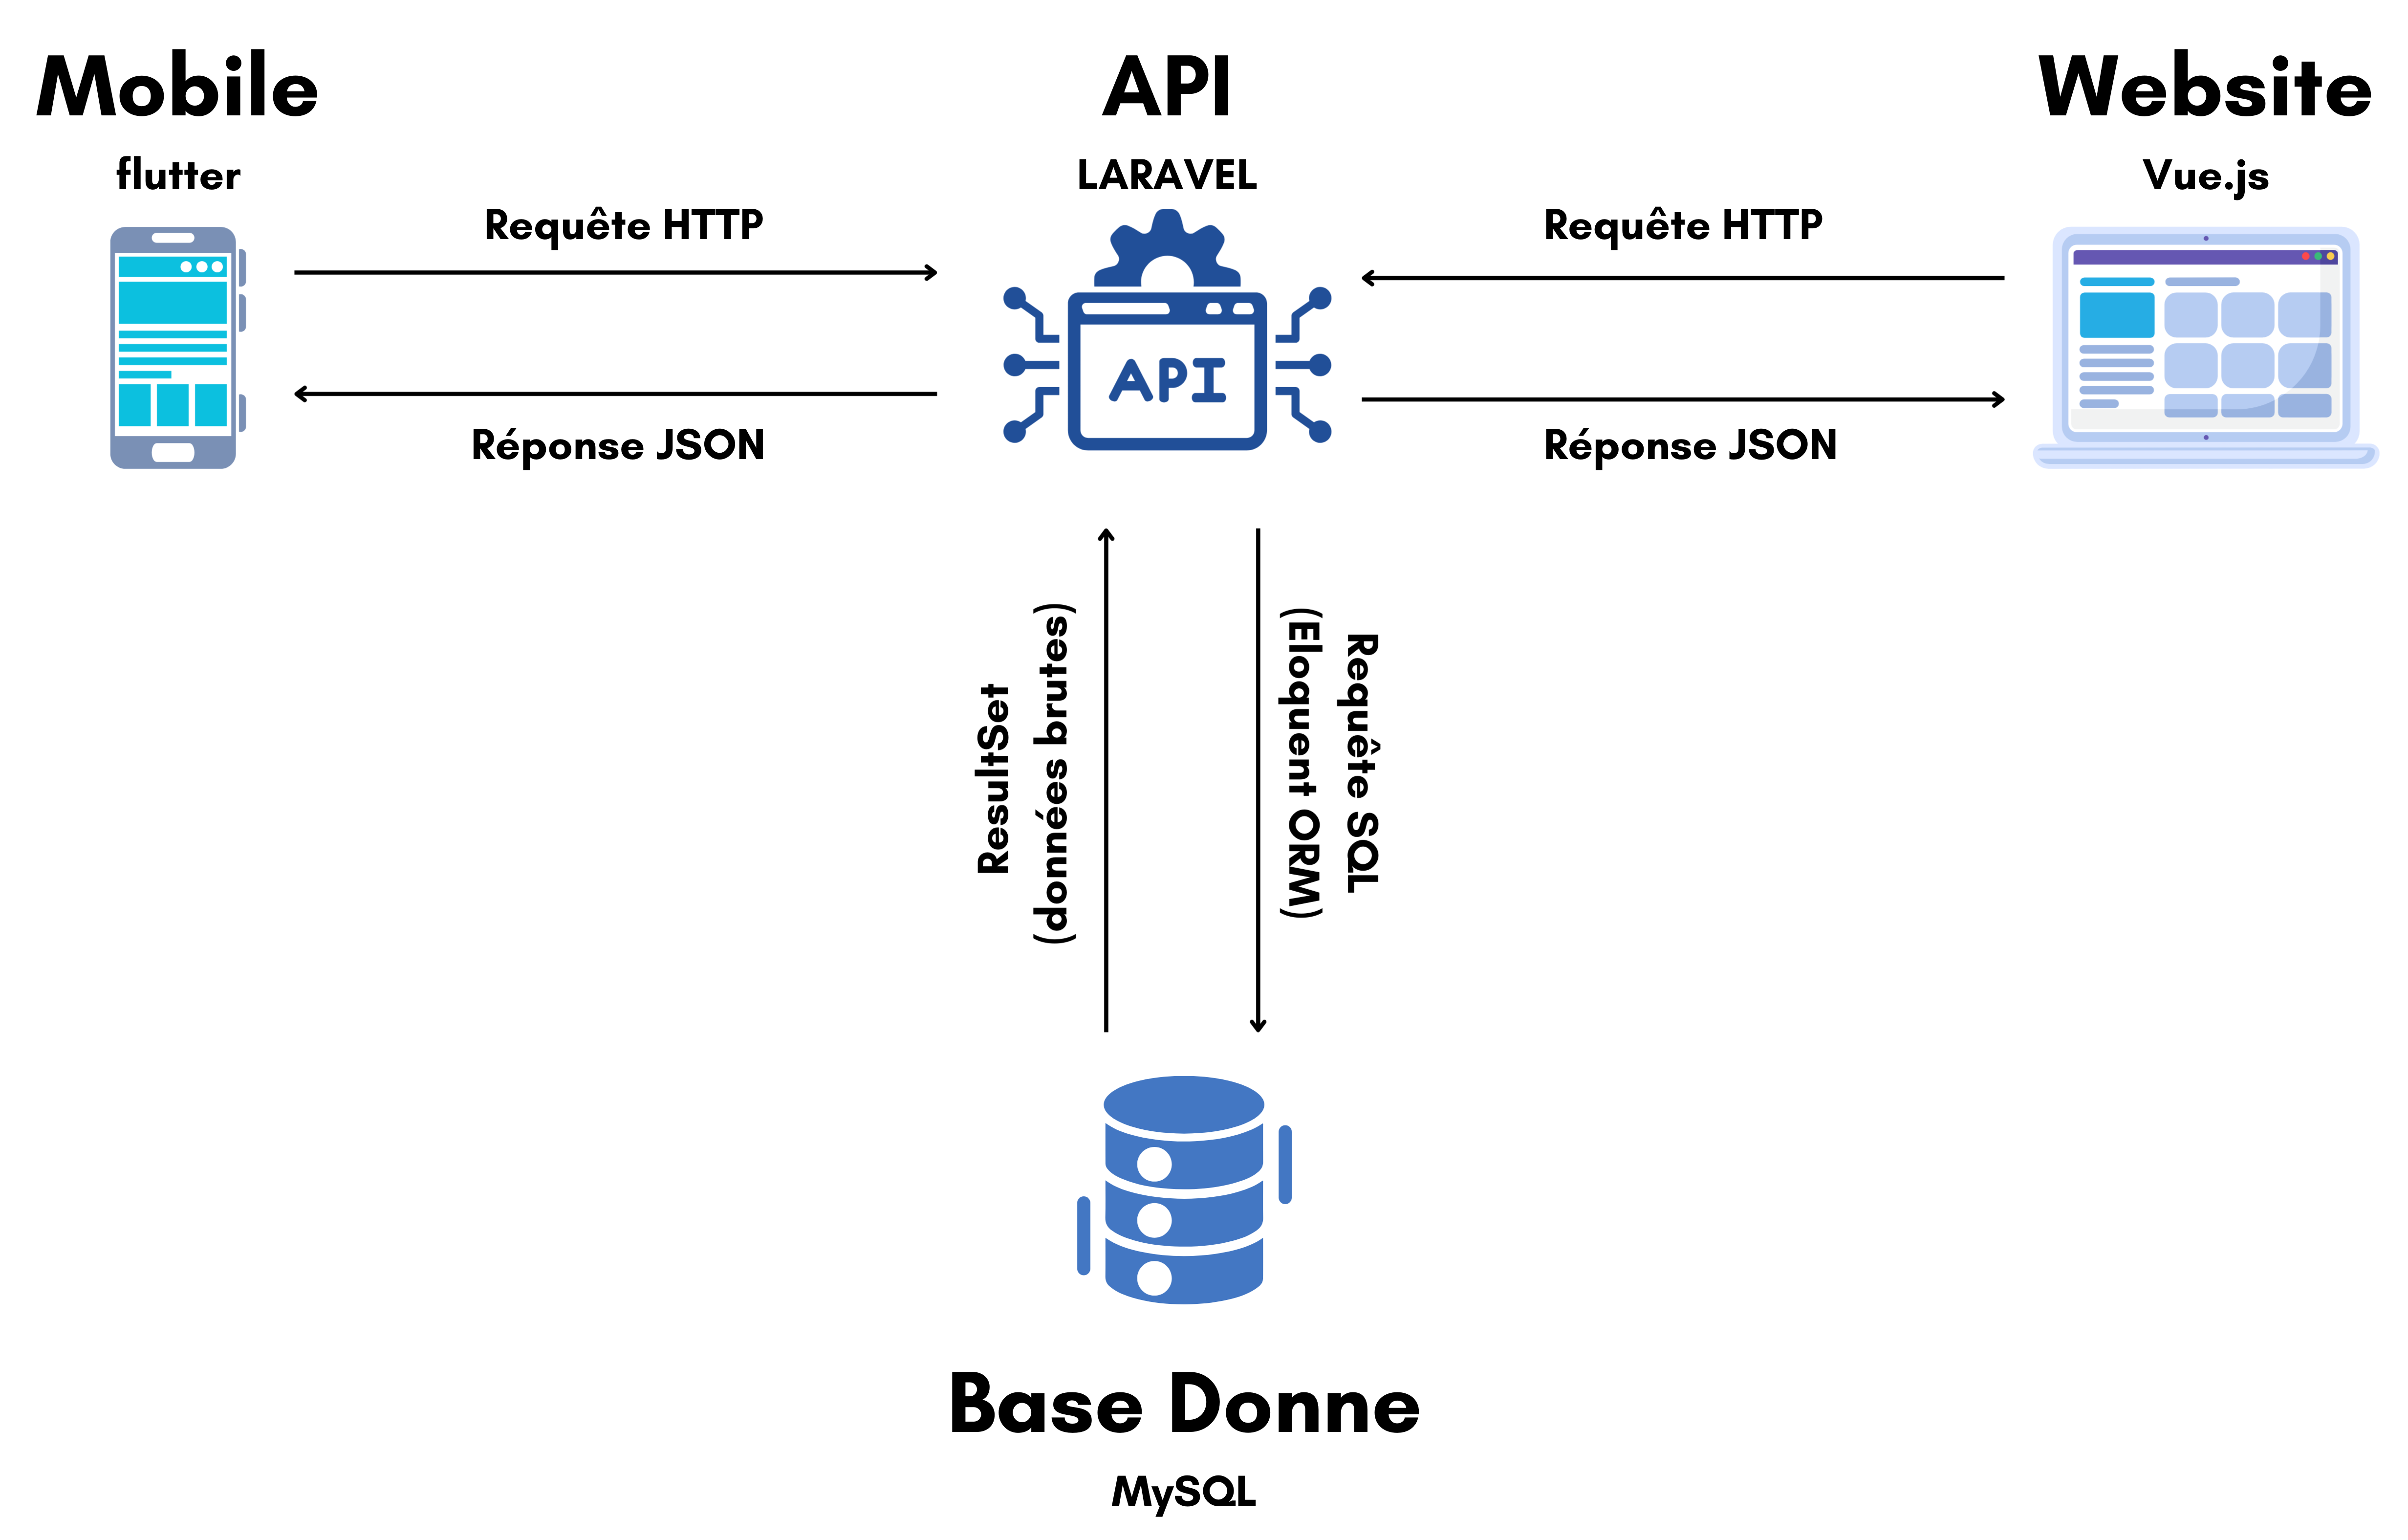
\includegraphics[width=0.9\linewidth]{architecture-overview.png}}{}
\caption{Architecture globale : web (React) et mobile (React Native) via API NestJS}
\label{fig:architecture-overview}
\end{figure}

% ============================================================
\chapter{Analyse, spécification des besoins et conception}

Ce chapitre présente l'analyse des besoins, les contraintes non-fonctionnelles et la conception du système (cas d'utilisation, diagrammes de classes et séquences).

\section{Analyse et spécification des besoins}

\subsection{Besoins fonctionnels}

Les besoins principaux identifiés sont :
\begin{itemize}
  \item Consultation des films et des séances disponibles.
  \item Recherche avancée et filtres (date, cinéma, genre).
  \item Sélection interactive des sièges avec vérification en temps réel.
  \item Paiement sécurisé et émission de billets numériques.
  \item Gestion des comptes utilisateurs (historique, annulations, préférences).
  \item Interface d'administration pour la gestion des films, salles et séances.
\end{itemize}

\subsection{Besoins non-fonctionnels}

Les contraintes comprennent la performance (latence faible pour la réservation), la fiabilité (consistance des états de réservation), la sécurité (protection des données personnelles et flux de paiement), l'évolutivité et la maintenabilité du code.

\subsection{Critères d'acceptation}

Exemples de critères : une réservation de siège doit être confirmée ou refusée immédiatement avec mise à jour atomique de la disponibilité ; un paiement doit générer un billet électronique consultable dans l'historique utilisateur.

\section{Conception du système}

\subsection{Identification des acteurs et cas d'utilisation}

Les acteurs principaux sont l'\\textbf{Utilisateur} (spectateur) et l'\\textbf{Exploitant} (gestionnaire de cinéma). Les cas d'utilisation incluent la recherche, la réservation, le paiement, la gestion des séances et la consultation des rapports de ventes.

\begin{figure}[H]
\centering
\IfFileExists{use-case-diagram.png}{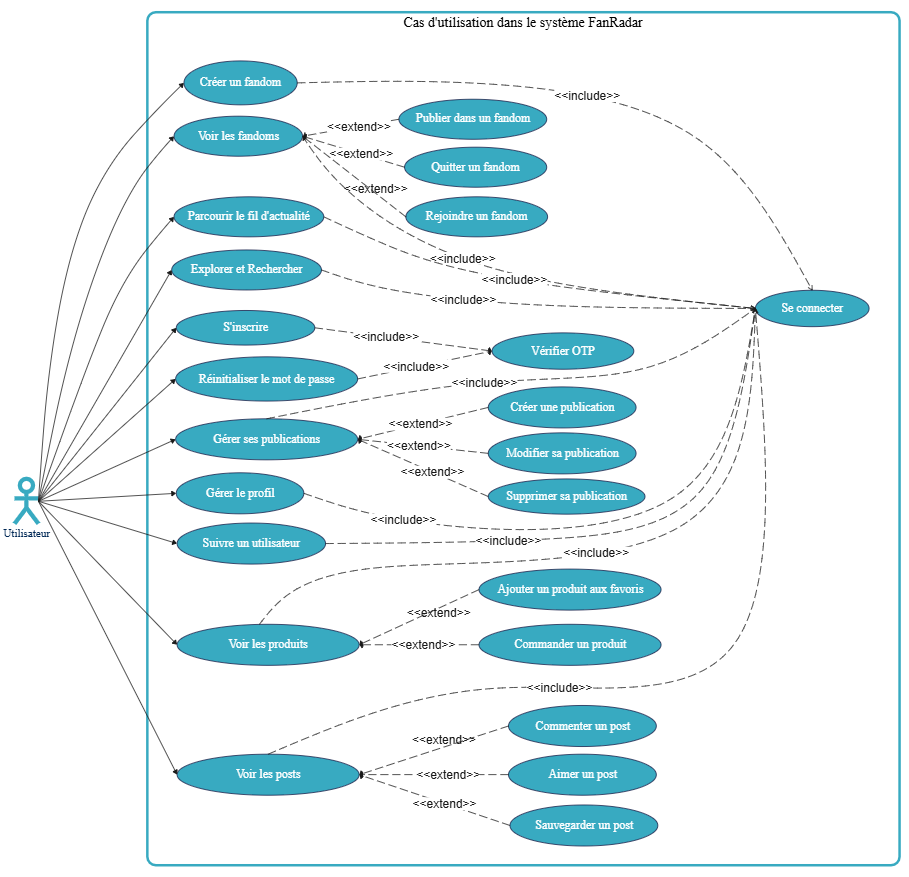
\includegraphics[width=1\textwidth]{use-case-diagram.png}}{}
\caption{Diagramme de cas d'utilisation du système CinePass}
\label{fig:use-case-diagram}
\end{figure}

\subsection{Diagramme de classes}

Les entités incluent \\\texttt{User}, \\\texttt{Film}, \\\texttt{Cinema}, \\\texttt{Room}, \\\texttt{Session}, \\\texttt{Seat}, \\\texttt{Reservation} et \\\texttt{Order}. La relation entre \\\texttt{Session} et \\\texttt{Seat} permet de modéliser l'occupation et la disponibilité.

\begin{figure}[H]
\centering
\IfFileExists{class-diagram.png}{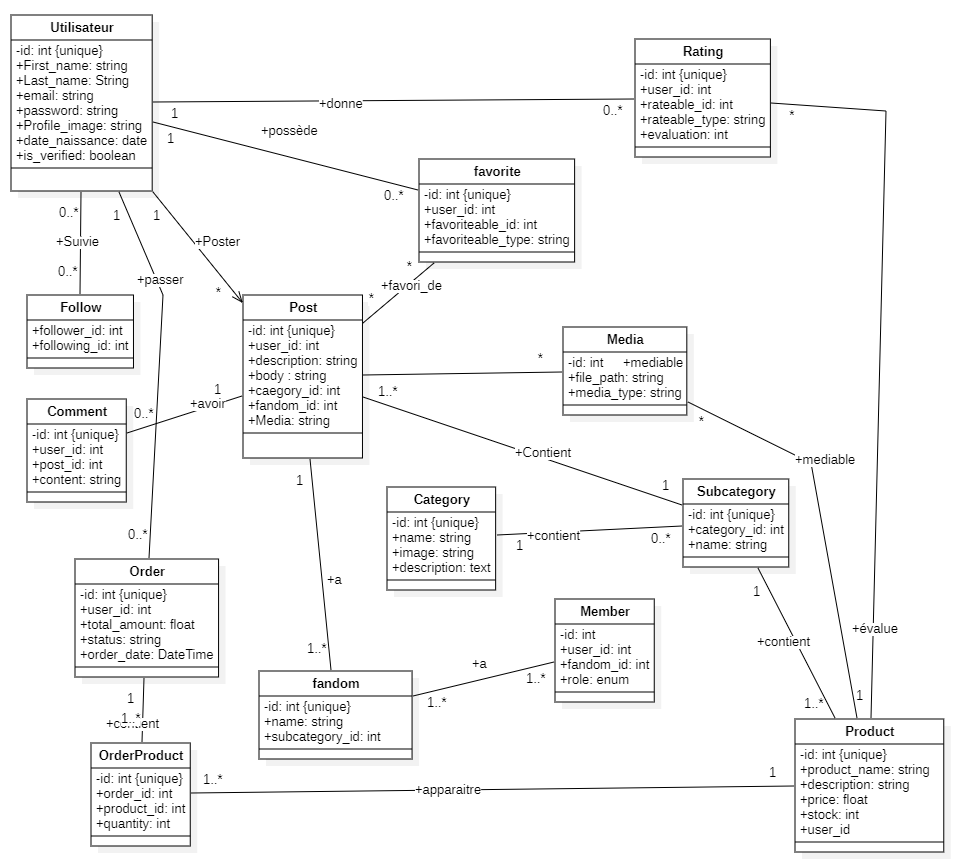
\includegraphics[width=1\textwidth]{class-diagram.png}}{}
\caption{Diagramme de classes du domaine CinePass}
\label{fig:class-diagram} 
\end{figure}

\subsection{Diagrammes de séquence}

Le flux de réservation comprend la sélection de la séance, le locking temporaire des sièges, le paiement puis la confirmation finale avec génération du billet.

\begin{figure}[H]
\centering
\IfFileExists{sequence-reservation.png}{\includegraphics[width=0.9\textwidth]{sequence-reservation.png}}{}
\caption{Processus de réservation et paiement}
\label{fig:sequence-reservation}
\end{figure}

% ============================================================
\chapter{Choix techniques et réalisation}

Ce chapitre décrit les décisions techniques et les réalisations effectives, y compris l'interface utilisateur, l'intégration backend et les tests.

\section{Architecture et choix technologiques}

\subsection{Architecture SPA}

L'application est conçue comme une SPA (Single Page Application) afin d'offrir une expérience fluide durant la navigation et la sélection des séances et sièges.

\subsection{React comme framework frontend}

React 18 a été retenu pour sa flexibilité, son écosystème (Vite, Tailwind) et ses performances. L'utilisation de TypeScript renforce la robustesse du code frontend.

\subsection{Environnement de développement}

\noindent\textbf{Langages utilisés.}\par
\vspace{0.3cm}

\noindent
\inlinetech{ts.png}{TypeScript}{Langage principal pour le frontend et le backend, apportant typage et maintenabilité.}

\noindent
\inlinetech{js.png}{JavaScript}{Utilisé côté client pour l'interactivité et les librairies.}

\noindent
\inlinetech{htmlcss.png}{HTML/CSS}{Structure et styles des pages, complétés par Tailwind CSS.}

\noindent\textbf{Frameworks et bibliothèques.}\par
\vspace{0.3cm}

\noindent
\inlinetech{react.png}{React}{Bibliothèque UI pour construire l'application web.}

\noindent
\inlinetech{nest.png}{NestJS}{Framework backend en TypeScript pour construire l'API REST.}

\noindent
\inlinetech{vite.png}{Vite}{Outil de build et serveur de développement pour le frontend.}

\noindent
\inlinetech{tailwind.png}{Tailwind CSS}{Framework utilitaire pour la mise en forme rapide et responsive.}

\noindent
\inlinetech{redux.png}{Redux Toolkit / Zustand}{Gestion d'état côté frontend selon les modules.}

\noindent\textbf{Outils de développement.}\par
\vspace{0.3cm}

\noindent
\inlinetech{vscode.png}{Visual Studio Code}{Éditeur principal.}

\noindent
\inlinetech{git.png}{Git}{Contrôle de version.}

\noindent
\inlinetech{github.png}{GitHub}{Hébergement et collaboration.}

\noindent
\inlinetech{postman.png}{Postman}{Tests d'API.}

\noindent
\inlinetech{nodejs.png}{Node.js}{Environnement pour les outils frontend.}

\noindent
\inlinetech{mysql.png}{MySQL/Postgres}{Système de gestion de base de données.}

\section{Réalisation et interfaces utilisateur}

\subsection{Architecture générale de l'interface}

La navigation met en avant la recherche de films, l'accès aux séances et la sélection des sièges. L'interface doit rester claire sur mobile comme sur desktop.

\subsection{Système de réservation}

Le module de réservation propose :
\begin{itemize}
  \item Une grille de sièges interactive montrant disponibilité et prix.
  \item Un verrouillage temporaire des sièges pendant le paiement.
  \item Gestion des réductions et cartes avantages.
  \item Génération d'un billet électronique après confirmation du paiement.
\end{itemize}

\subsection{Gestion des commandes et historique}

L'utilisateur dispose d'un historique de ses réservations, statuts et billets téléchargeables.

% ============================================================
\chapter*{Conclusion générale}
\addcontentsline{toc}{chapter}{Conclusion générale}

Le projet CinePass a permis de concevoir et développer une plateforme de billetterie fonctionnelle répondant aux besoins de réservation, de paiement et de gestion des salles. Le travail a renforcé les compétences en architecture frontend React, intégration d'API NestJS et gestion des états critiques pour les réservations en temps réel.

Les améliorations futures incluent l'optimisation des performances en charge élevée, l'ajout d'analyses avancées et l'intégration d'un système de fidélité enrichi.

% ============================================================
\chapter*{Bibliographie et webographie}
\addcontentsline{toc}{chapter}{Bibliographie et webographie}

\section*{Webographie}

Documentation React : \url{https://reactjs.org/}. NestJS Documentation : \url{https://docs.nestjs.com/}. Vite Documentation : \url{https://vitejs.dev/}. Tailwind CSS Documentation : \url{https://tailwindcss.com/docs}.

\end{document}
